\section{Aplicación de ejemplo}

Para comprender mejor esta problemática veamos un ejemplo. Supongamos una simple
aplicación, donde los clientes de un banco pueden transferir dinero de
una cuenta a otra. Al realizar una transferencia, hay que extraer el monto
indicado de una cuenta, y depositarlo en otra. 
Al ejecutar cualquiera de estas dos operaciones se pueden producir errores,
como por ejemplo, que no haya saldo saldo suficiente, o que el depósito supere
el máximo permitido.
La  figura \ref{example} muestra el diagrama de clases de la aplicación de
ejemplo

	\begin{figure}[h]
		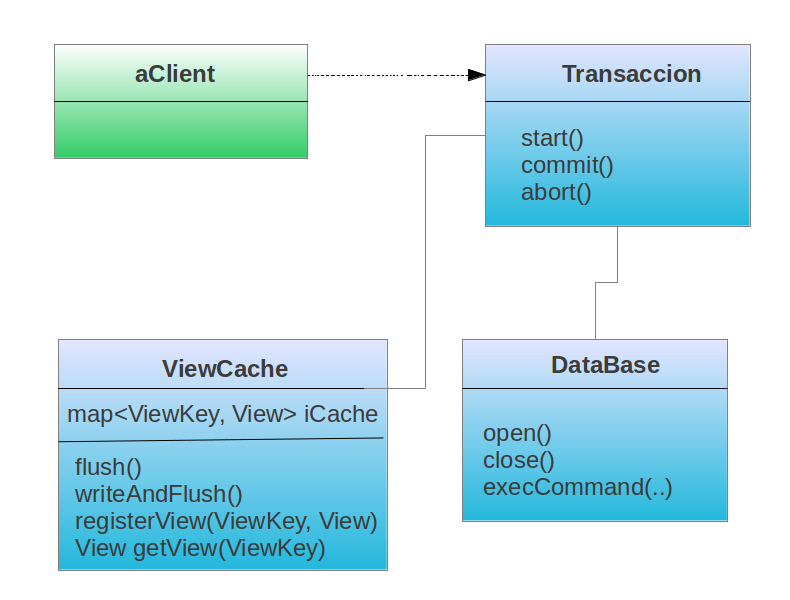
\includegraphics{img/objectTransaction}
		\caption{Diagrama UML de la aplicación de ejemplo}
		\label{example}
	\end{figure}	


El sistema me permite realizar múltiples transferencias a la vez y por último
realizar la confirmación o la cancelación de todas ellas. También brinda la posibilidad
de realizar múltiples transacciones, por ejemplo, en la edición de un cliente,
se puede editar, eliminar o crear cuentas. A su vez se puede hacer una
transferencia a otra cuenta. En cada una de esas operaciones se esta
trabajando en dentro de una transacción. y las operaciones pueden ser
canceladas por unidad, es decir, se cancelan o se confirman por transacción.

Caso de uso 1: transferir plata.
Tres ventajas:
- queda más simple
- menos posibilidad de mandármela
- concurrencia.

Poner el código como queda.

Caso de uso 2: transferencias múltiples.
muchas transferencias en una única transacción\ldots fijate si sale algo y si no
lo volamos.

\section{Nuestra herramienta: }

En esta sección se explica como se llevó a cabo la implementación de la solución
propuesta en la Sección \ref{sec:Solucion}, y cumpliendo el objetivo detallado
en la Sección \ref{sec:Objetivo}. Se desarrollaron dos herramientas
fundamentales para lo planteado. \emph{Pure Objects Observable} (POO) para atacar a la
problemática de la observabilidad y \emph{Pure Object Transaction} (POT) para
atacar a la problemática transaccional.
	
	\subsection{Selección de un framework de aspectos}  
	Un primer paso para la implementación de la herramienta fue la selección de una
	tecnología que permitiera desarrollar con programación orientada a aspectos.
	Se evaluaron dos frameworks para resolver nuestro problema.
	Uno es Javassist \cite{??} y el otro AspectJ \cite{KiczalesHHKPG01}.

	\medskip 
	Encontramos AspectJ es una herramienta de más alto nivel, que extiende
	el lenguaje Java agregando construcciones específicas para trabajar con
	los conceptos de la teoría de programación orientada a aspectos.
	Por otro lado AspectJ requiere que el programador usuario de nuestro framework
	utilice un compilador específico. Consideramos que esta característica es muy
	negativa, por condicionar el entorno de trabajo de los usuarios de nuestra
	herramienta.
	En cambio Javassist agrega los aspectos al momento de la carga de las clases,
	sólo requiere que utilicemos un \emph{ClassLoader} específico.

	Elegimos Javaassist por su menor impacto para el programador que utilice el
	framework como usuario.
	Para minimizar los problemas asociados a utilizar un framework de tan bajo
	nivel desarrollamos una herramienta que simplifica su uso agregando algunas
	abstracciones útiles. Esta herramienta se describe en la sección siguiente.

	\subsection{Desarrollo de Aspect for Pure Objects}

	El framework Javassist permite modificar directamente el \emph{bytecode} de
	una clase en el momento de cargarla.
	Por ser de tan bajo nivel es uno de los frameworks de aspectos más poderosos,
	pero a su vez el código se hace poco entendible.
	Por eso se desarrolló una herramienta llamada \emph{Aspect for Pure Objects} (APO), 
	que permite configurar aspectos utilizando conceptos de más alto nivel y
	aplicárselo a un grupo de objetos.
	
	Acá agregar un poco de código\ldots contar un poco más la herramienta.


	\subsection{Pure Object Transaction} 
		Pure Object Transaction es la herramienta que resulve el problema
		transaccional. Basado en una implementación hecha por
		Nicolás Passerini y Javier Fernandes. Se utilizo los mismos conceptos en esta
		implementación, pero utilizando el APO.
		 
		El framework intercepta todas las lecturas	y escrituras de los atributos de un
		objeto.	Insertando código al momento de la carga de la clase.
		Se remplaza el acceso al atributo, tanto de lectura como escritura, y se lo
		delega al administrador de las transacciones, donde se guarda la información
		en una estructura [Objeto, [Atributo, Valor]].
		
		\medskip
		
		En la primera implementación no interceptaba las operaciones sobre los
		atributos de Collecciones, ya que Java impide modificar sus clases, por
		ende no se puede agregarle dicho aspecto.
		Por ejemplo al agregar un elemento a la collección, se re está realizando una
		nueva asignacción, sino que se modifica la colección. Entonces el framework no
		puede mantener el registro de las modificaciones y al realizar un
		\emph{roolback} los cambios no se revierten.
		En la version actual se resolvio este problema, reemplazando la implentacion
		de la collección elegida por el usuario, por una implementada especialmente
		para resolver este problema.
		
		\medskip
		
		El contexto de la transacción esta asociado a un solo \emph{thread}. Esto
		permite manejar la concurrencia en el acceso a la información de los objetos. 
		Soportando transacciones anidadas, donde cada transacción hija hereda el estado
		de su padre, y al momento de hacer el \emph{commit} en la sub-transacción, sus
		cambios son impactados en la transacción padre.
		Por esta forma de implementación, la identidad del objeto se mantiene, ya que
		el objeto no se modifica ni se clona, solo se cambia el acceso a sus
		atributos.
		
		Para agregarle este aspecto a una clase se utiliza la \emph{Annotation}
		\emph{Transactional }
				
		\begin{figure}[h]
				\begin{lstlisting} 
					@Transactional
					public class Client extends Entity {
					}
				\end{lstlisting}
			\caption{Ejemplo de uso del Aspecto Transaccional}
			\label{pot}
		\end{figure}  

	\subsection{ Pure Observable Objects}
			
		Pure Observable Objects es el framework que resulve el problema de la
		observabilidad panteado anteriormente. En su implementación interna lo que
		hace el aspecto es agregar un atrubuto \emph{changeSupport} del tipo
		\emph{<<PropertySupport>>} al objeto que se va a convertir en Observable. Pero
		su implementación se obtiene del el archivo de configuración.
		
		Luego se agrega los siguientes métodos para completar su objetivo.
		El primero es el \emph{firePropertyChange} que es el que notifica a los
		Observadores que una propiedad ha cambiado.	Luego le agregamos
		\emph{addPropertyChangeListener} y \emph{removePropertyChangeListener} para
		poder agregar y remover Observadores para que escuchen sus cambios.
		
		Para agregarle este aspecto a una clase se utiliza la \emph{Annotation}
		\emph{Observable}
		
	\begin{figure}[h]
		\begin{lstlisting} 
			@Observable
			public class Client extends Entity {
			}
		\end{lstlisting}
		\caption{Ejemplo de uso del aspecto observable}
		\label{poo}
	\end{figure}  
		


	
\subsection{Integración de aspectos con el Arena}
	En Arena se integró los dos aspectos, el Observable y el transaccional, con el
	fin de que los objetos de dominio sean puros, y que no tengan la noción de
	eventos, ni transacciones, y así poder bindearlos con los componentes de de la
	interfaz gráfica. Y al cancelar la edición poder revertir los cambios
	transparéntenme.
	
	Para ello se tubo que asociar una transacción con una ventana, en el caso mas
	especifico con la clase \emph{TransactionalDialog}. A su vez también tenemos
	vinculado los eventos del dominio junto con la ventana y la transacción.
	Se implemento tres niveles de aislamiento de los eventos,  \emph{Fire All},
	\emph{Fire Committed} y \emph{Fire olnly in my transaction};
	
	\begin{description}
		\item[\emph{Fire All}] Todos los eventos disparados por el dominio son
		escuchados, sin importar si están en una transacción.
	
		\item[\emph{Fire Committed}] Solo se escucha los eventos de las transacciones
			comiteadas
		
		\item[\emph{Fire olnly in my transaction}] solo se escucha los eventos que
			ocurren dentro de su translación.
	
	 \end{description}
	 
	Framework permite permite poder tener uno, otro o ambos aspecto. Se puede poner
	los dos \emph{Annotation} \emph{Observable} y \emph{Transactional} como vimos
	previamente, o ponerle \emph{TransactionalAndObservable} que es una union de
	ambos.
	
	\begin{figure}[h]
		\begin{lstlisting} 
			@TransactionalAndObservable
			public class Client extends Entity {
			}
		\end{lstlisting}
		\caption{integración de ambos aspectos}
		\label{TandO}
	\end{figure}  
	
	 

	
	\subsection{Otras mejoras al Arena}
	La integración se realizo con el lenguaje de programación Scala
	\cite{ref}. Para llevar al cabo la integración se agregó algunas
	mejoras en el Arena. 
	Algunas mejoras fueron:
	\begin{description}
	  \item[Monitor de Transacciones]
		 Con arena también se desarrolló un \emph{Monitor de Transacciones}, que 
		 muestra el estado actual de la transacción, incluyendo las transacciones
		 anidadas. Mostrando los objetos afectados por la transacción y los
		 atributos se modificaron.
	  \item[Nuevos componentes] Se Implementaron algunas estructuras visuales como
	  Arboles y Listas.
	  \item[Bindinds Anidados] Se implemento bindings para las propiedades
	  anidadas de los objetos.
	\end{description}
